
\documentclass[final,11pt,a4paper,twocolumn,oneside]{article}
% \documentclass[11pt,a4paper]{article}
% \documentclass[5p,twocolumn,sort&compress]{elsarticle}
% \documentclass[final,5p,times,twocolumn,sort&compress]{elsarticle}
% \documentclass[a4paper,12pt]{report}

\usepackage[utf8]{inputenc}

\usepackage{amsmath}
\usepackage{amsfonts}
\usepackage{amssymb}
\usepackage{graphicx}
\usepackage{array}
\usepackage{booktabs}
\usepackage{float}
\usepackage{newclude}
\usepackage{bm}
\usepackage{pdfpages}

\usepackage[binary-units=true]{siunitx}
\usepackage[colorlinks,allcolors=blue]{hyperref}
\usepackage[font={small,it}]{caption}
\usepackage[font={small,it}]{subcaption}
\usepackage[hmargin={0.7in,0.6in},vmargin={0.9in,1in}]{geometry}

\edef\restoreparindent{\parindent=\the\parindent\relax}
\usepackage{parskip}
\restoreparindent

\usepackage{biblatex}
\bibliography{references}

\usepackage{mathtools}
\DeclarePairedDelimiter{\abs}{\lvert}{\rvert}

\interfootnotelinepenalty=10000
\raggedbottom

\setcounter{topnumber}{8}
\setcounter{bottomnumber}{8}
\setcounter{totalnumber}{8}

% \sisetup{range-units=single}
% \sisetup{range-phrase=\kern 0.08333em--}

\title{\bfseries Simulating the Measurement of the\\
Electron Beam Emittance at AWAKE}
\author{Patrick~Chin}
% \author[ucl]{P.~Chin}
% \author[ucl]{E.~Simpson~Dore}
% \author[ucl]{L.~Deacon}
% \author[ucl]{F.~Keeble}
% \author[ucl]{S.~Jolly}
% \author[ucl]{M.~Wing}
% \address[ucl]{UCL, Gower Street, London WC1E 6BT, UK}
% \date{\today}

\begin{document}

\twocolumn[
	\begin{@twocolumnfalse}

% \begin{titlepage}
% \center
% \textbf{\LARGE Phase Ordering Kinetics \& Infinite Rapid Quenching of the Compact KPZ Equation for Polariton Condensates}\\[5.0cm]
% \textsc{\textit{Author: Nisha Lad}}\\[0.15cm]
% \textsc{\textit{Supervised by Dr. Marzena Szymańska}}\\[0.15cm]
% \textsc{\textit{\& Dr. Alejandro Zamora}}\\[5.0cm]
% %\LARGE Project Report \\[2cm]
% \textbf{\large MSci Physics}\\[0.1cm]
% \large Department of Physics \& Astronomy \\[0.1cm]
% \large University College London, U. of London \\[1cm]
% \normalsize \today
% \vfill
% \end{titlepage}

		\vspace*{18em}
		\maketitle
		\thispagestyle{empty}
		\vspace*{5em}
		\begin{center}
			Department of Physics \& Astronomy, \\
			University College London \\
			% Gower Street, London, WC1E 6BT \\
			\vspace*{6em}
			Supervised by Prof.~M.~Wing \\ \& Dr.~S.~Jolly \\
		\end{center}

	\end{@twocolumnfalse}
]

\clearpage
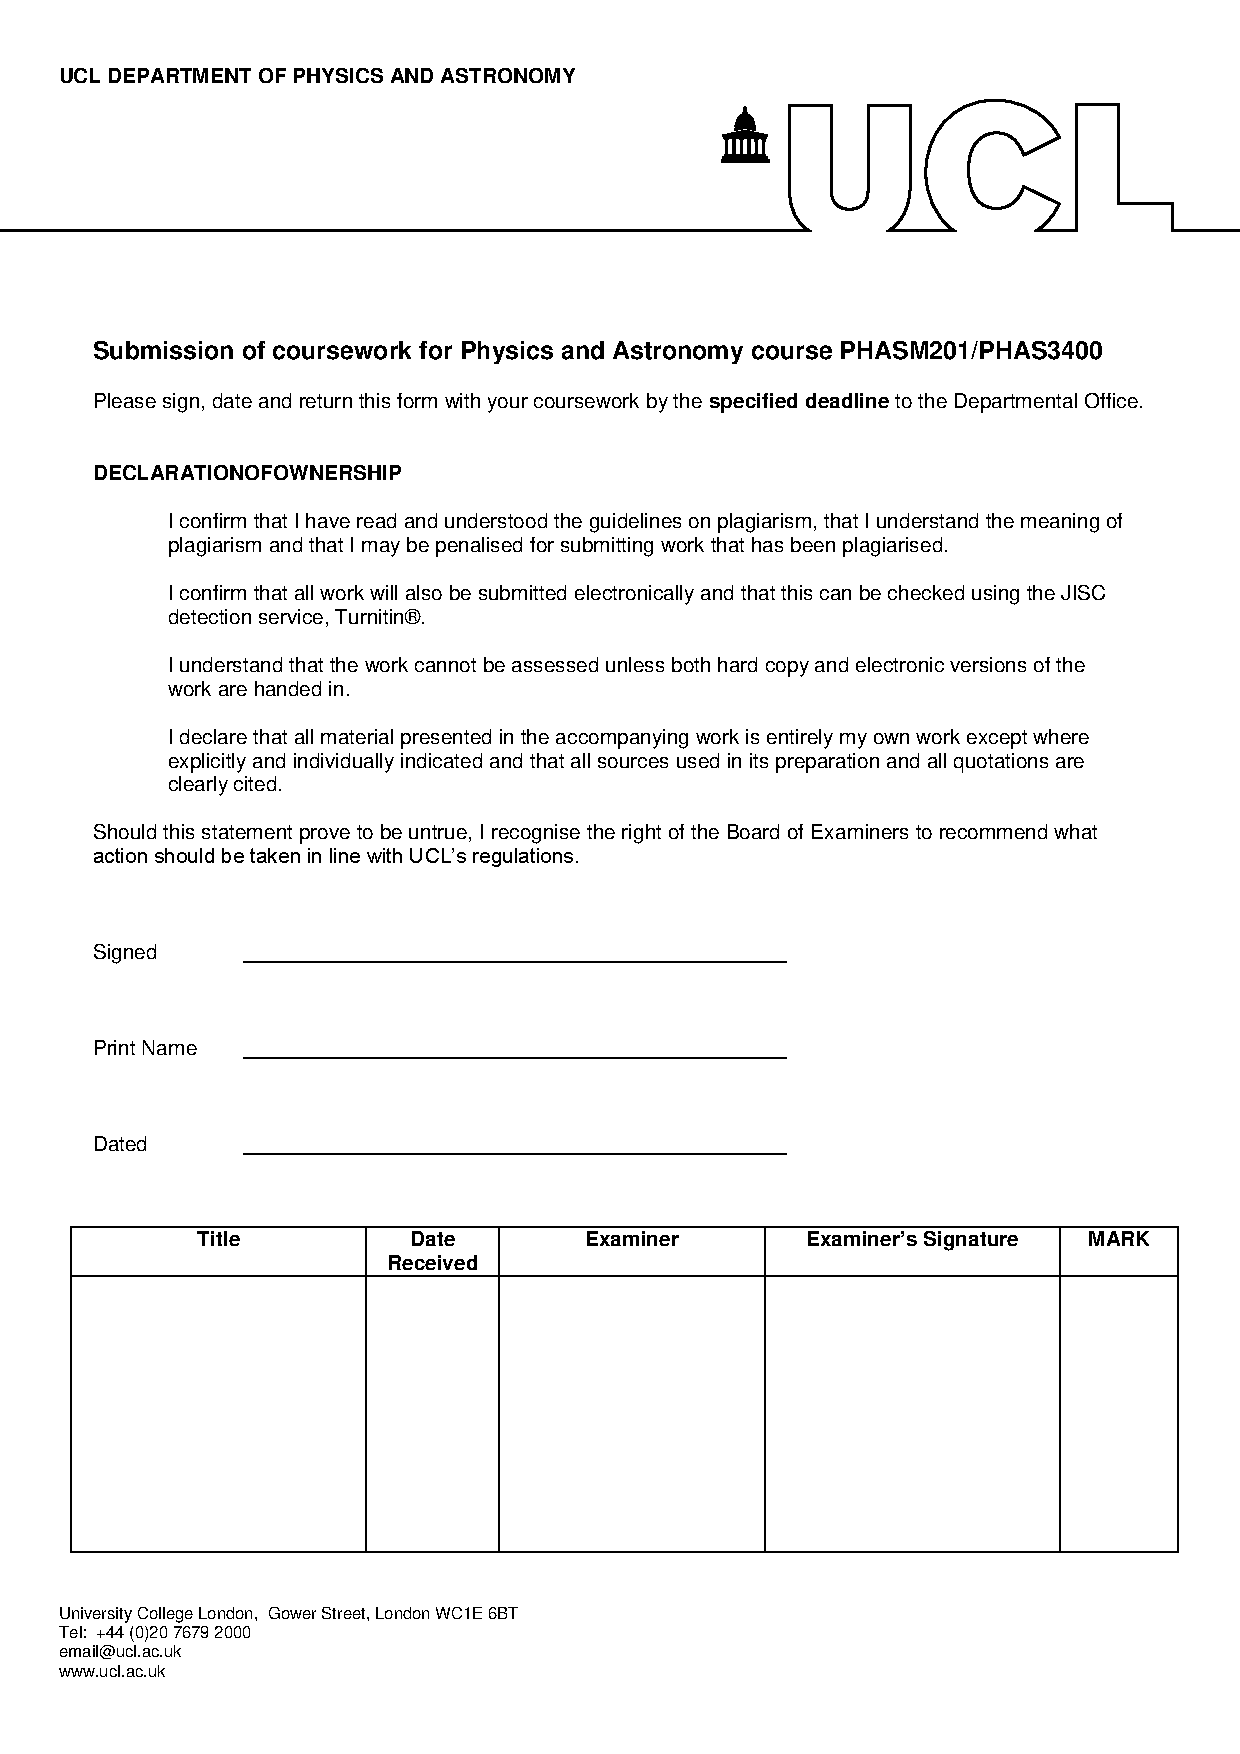
\includepdf{declaration.pdf}

\twocolumn[
	\begin{@twocolumnfalse}
	\thispagestyle{empty}
	\vspace*{18em}

% \begin{frontmatter}
	% \begin{abstract}

		\begin{center}
			\section*{Abstract}
		\end{center}

		In preparation for runs at AWAKE in CERN, simulations of the beam and
		measurement of beam parameters with a spectrometer were carried out.
		This was done in order to investigate how the spectrometer behaves under
		changes to experimental parameters. The energy spreads of the beam were
		tested and a percentage energy spread of \SI{4}{\percent} was found to
		be the cutoff point at which measurements become reliable. Emittance
		values were tested and emittances above \SI{e-5}{\meter\radian} were
		found to be inaccurate.  Background photon values up to \num{e4} times
		the expected background were simulated, showing accurate measurements up
		to a factor of \num{\sim4e2}, above which the measured emittance
		deviated significantly from the true value.

	% \end{abstract}

		% \begin{keyword}
		% 	plasma wakefield \sep
		% 	spectrometer \sep
		% 	emittance \sep
		% 	electron beam \sep
		% 	self-modulation instability
		% \end{keyword}
% \end{frontmatter}

	\end{@twocolumnfalse}
]

\clearpage
\clearpage
\twocolumn[
	\begin{@twocolumnfalse}
		\thispagestyle{empty}
		\hypersetup{allcolors=black}
		\tableofcontents
	\end{@twocolumnfalse}
]
\clearpage

% \pagenumbering{arabic}
\include*{introduction}
\include*{awake}
\include*{spectrometer}
\include*{theory}
\include*{simulation}
\include*{results}
\include*{conclusion}
% 
% % \appendix
% \begin{appendices}
% \part{Code}
% \end{appendices}


\clearpage
% \section*{References}
% \bibliographystyle{ieeetr}
% \bibliography{references}
\printbibliography

\end{document}

